 % -*- root: ../main.tex -*-
\documentclass[../main.tex]{subfiles}
\begin{document}

\chapter{Publications}\label{chap:publications}

\clearpage
\newpage

% ================================================

\section{Mécanismes d'action des récepteurs aux hormones thyroïdiennes durant le développement : Lessons retenues des études sur les amphibiens}\label{sec:bba-review}

\begin{abstract}
Les \glspl{tr} jouent un rôle critique durant le développement des vertébrés.
Cependant, leur mécanismes d'action \textit{in vivo} reste peu exploré.
Cette revue catalogue certains des résultats obtenus dans le contexte de la métamorphose des amphibies sur les fonctions développementales des \glspl{th} et des \glspl{tr} et leur mécanismes associés.
\par
Un modèle de double fonction de \gls{tr} pour le développement des Anoures a été proposé il y a près d'une décade.
Selon ce modèle, \gls{tr} non lié à son ligand recrute des complexes co-répresseurs – contenant des désacétylases d'histones – au niveau de gènes cibles des \glspl{ht} durant la pré-métamorphose pour réprimer l'expression de ces gènes et empêcher la métamorphose prématurée.
Par la suite, quand les \glspl{ht} sont disponibles, \gls{tr} lié au ligand recrute des complexes co-activateurs – contenant des modificateurs d'histones et des remodeleurs de la chromatine – pour cette fois activer l'expression de ces même gènes et induire les changements associés à la métamorphose.
Ces complexes peuvent altérer la structure de la chromatine par déplacement ou éviction des nucléosomes et la modification d'histones, contribuant au recrutement de la machine transcriptionnelle et à l'activation de gènes.
\par
Les mécanismes moléculaires impliqués dans ce modèle sont très probablement transposables à des modèles mammaliens.
\end{abstract}

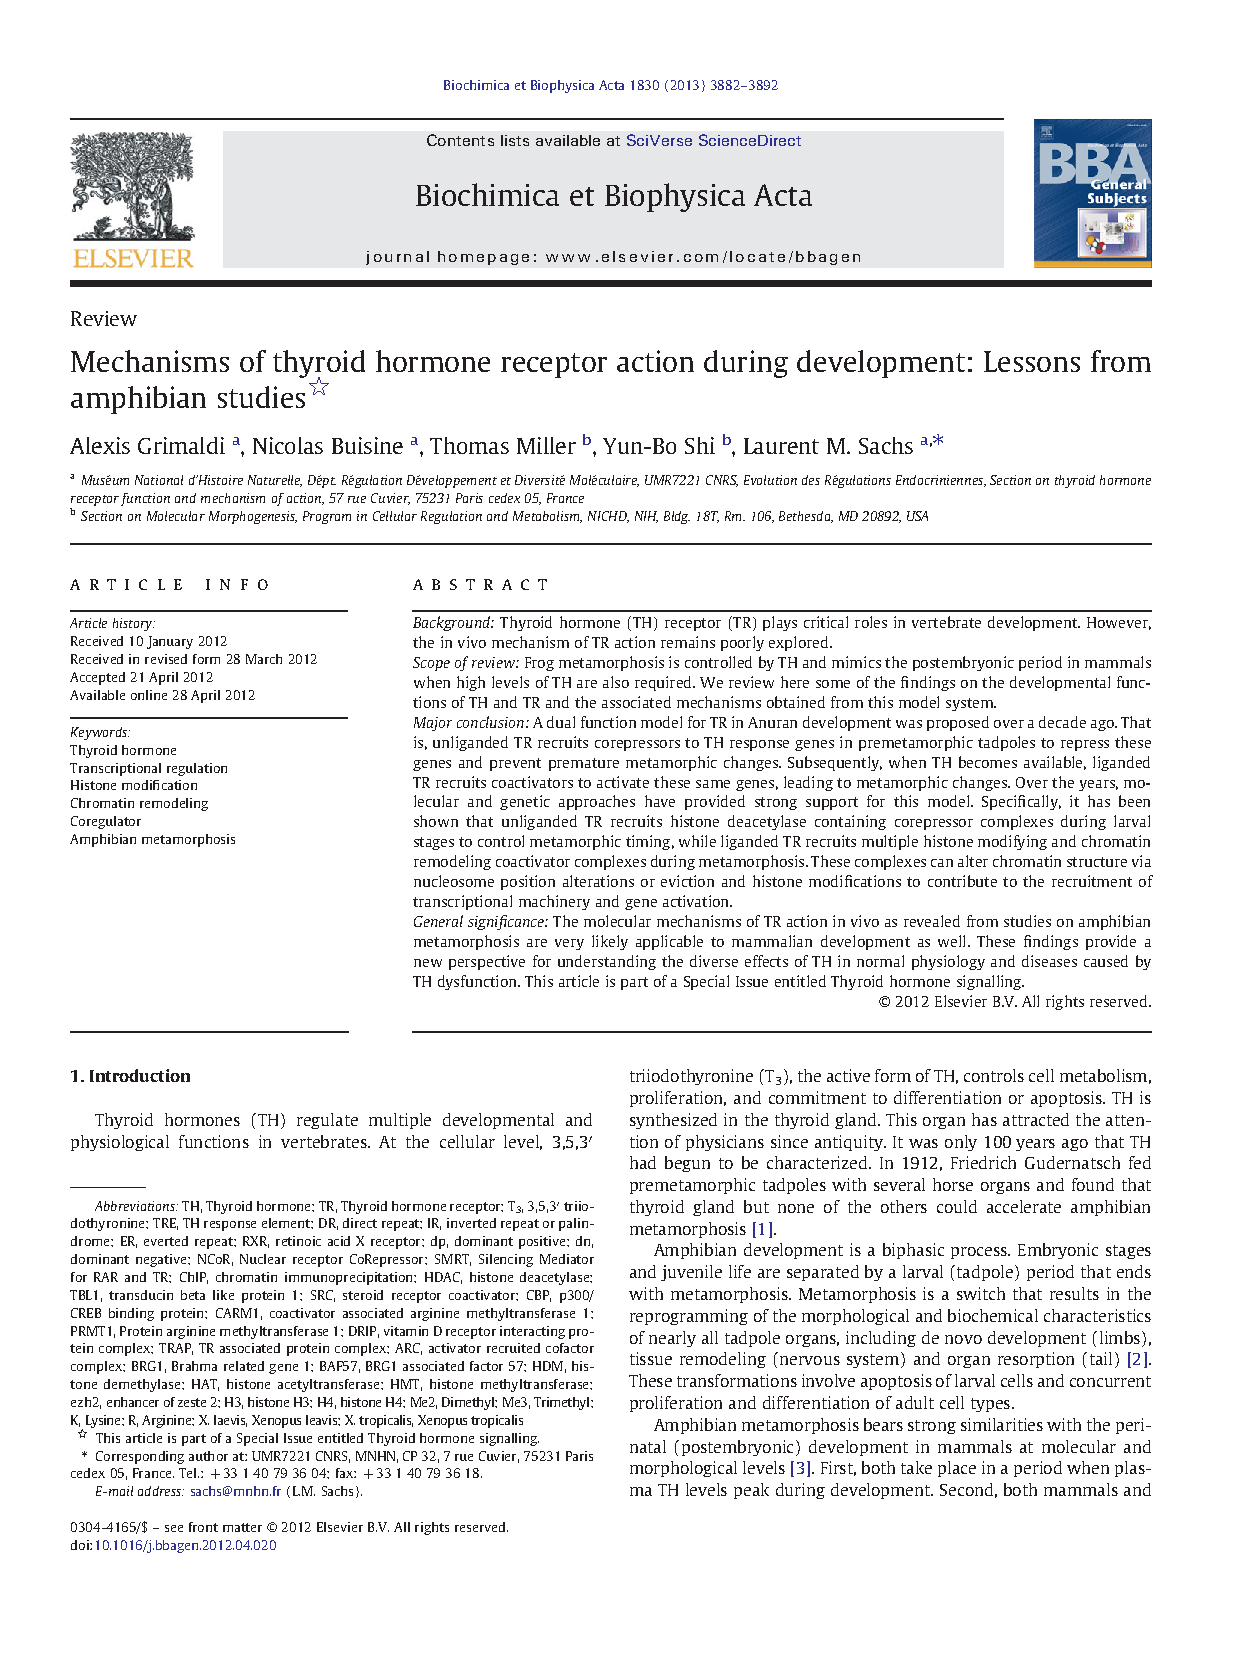
\includepdf[pages={-}]{Publications/bba-review.pdf}

% ====================================================

\clearpage
\newpage

% ====================================================

\section{Les technologies de séquençage à haut débit vont métamorphoser l'analyse de la fonction des récepteurs aux hormones thyroïdiennes pendant le développement de l'amphibien}\label{sec:ctdb-review}

\begin{abstract}

Amphibian metamorphosis is marked by dramatic thyroid hormone (T3)-induced changes including de novo morphogenesis, tissue remodeling, and organ resorption through programmed cell death.
These changes involve cascades of gene regulation initiated by thyroid hormone (TH).
TH functions by regulating gene expression through TH receptors (TR).
TR are DNA-binding transcription factors that belong to the steroid hormone receptor superfamily.
In the absence of ligand, TR can repress gene expression by recruiting a corepressor complex, whereas liganded TR recruits a coactivator complex for gene activation.
Earlier studies have led us to propose a dual function model for TR during development.
In premetamorphic tadpoles, unliganded TR represses transcription involving corepressors.
During metamorphosis, endogenous T3 allows TR to activate gene expression.
To fully understand the diversity of T3 effects during metamorphosis, whole genome analysis of transcriptome and mechanism of TR action should be carried out.
To this end, the new sequencing technologies have dramatically changed how fundamental questions in biology are being addressed and is now making the transition from technology development to being a standard for genomic and functional genomic analysis.
This review focuses on the applications of high-throughput technologies to the field of amphibian metamorphosis.

\end{abstract}

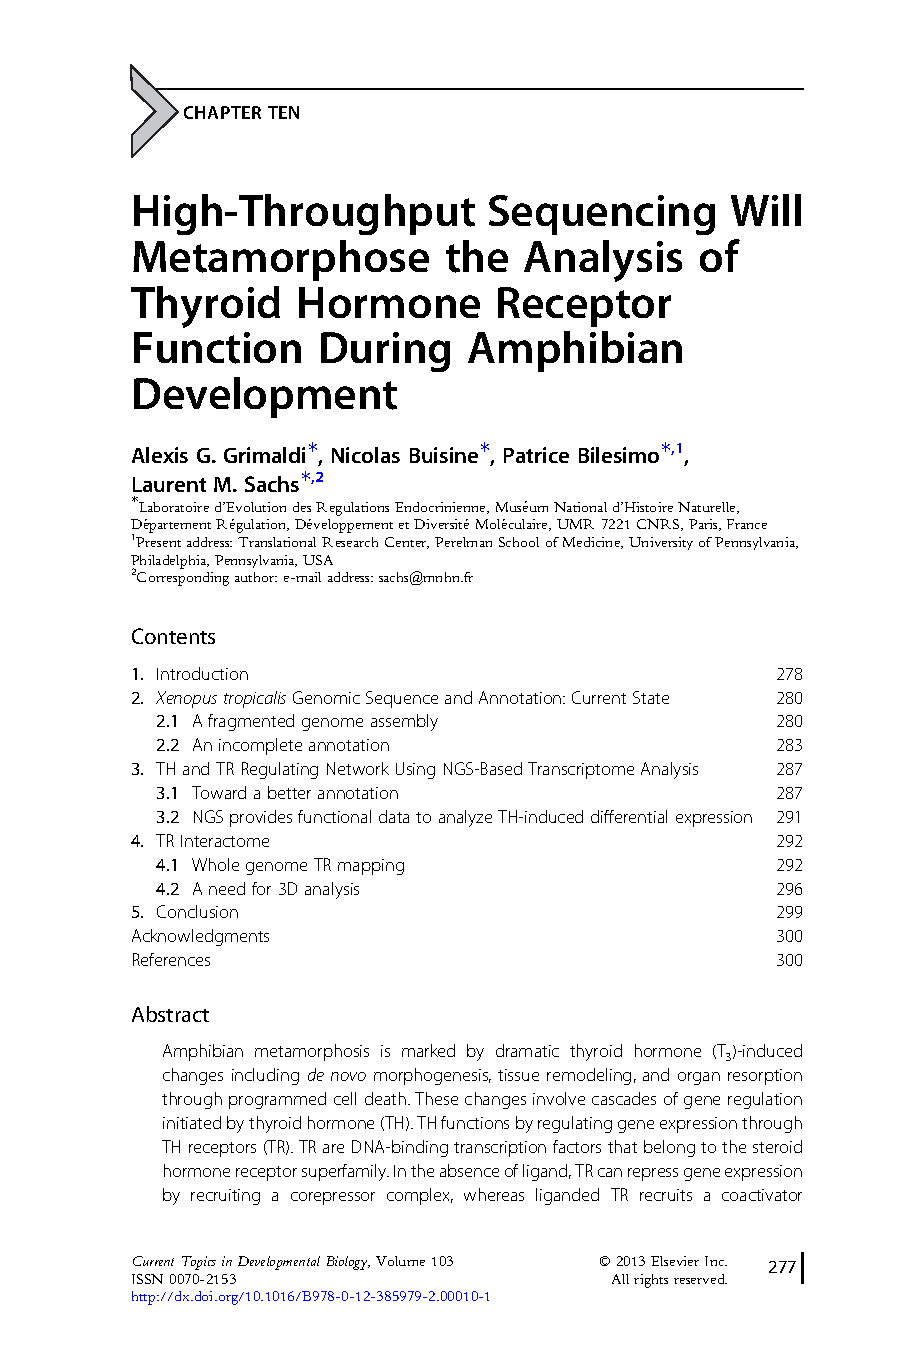
\includepdf[pages={-}]{Publications/ctdb-review.pdf}

\clearpage
\newpage

\section{Re-assembly and re-annotation of the Xenopus tropicalis genome for in vivo ChIA-PET analysis}\label{sec:buisine2014}

\begin{abstract}

Abstract

\end{abstract}

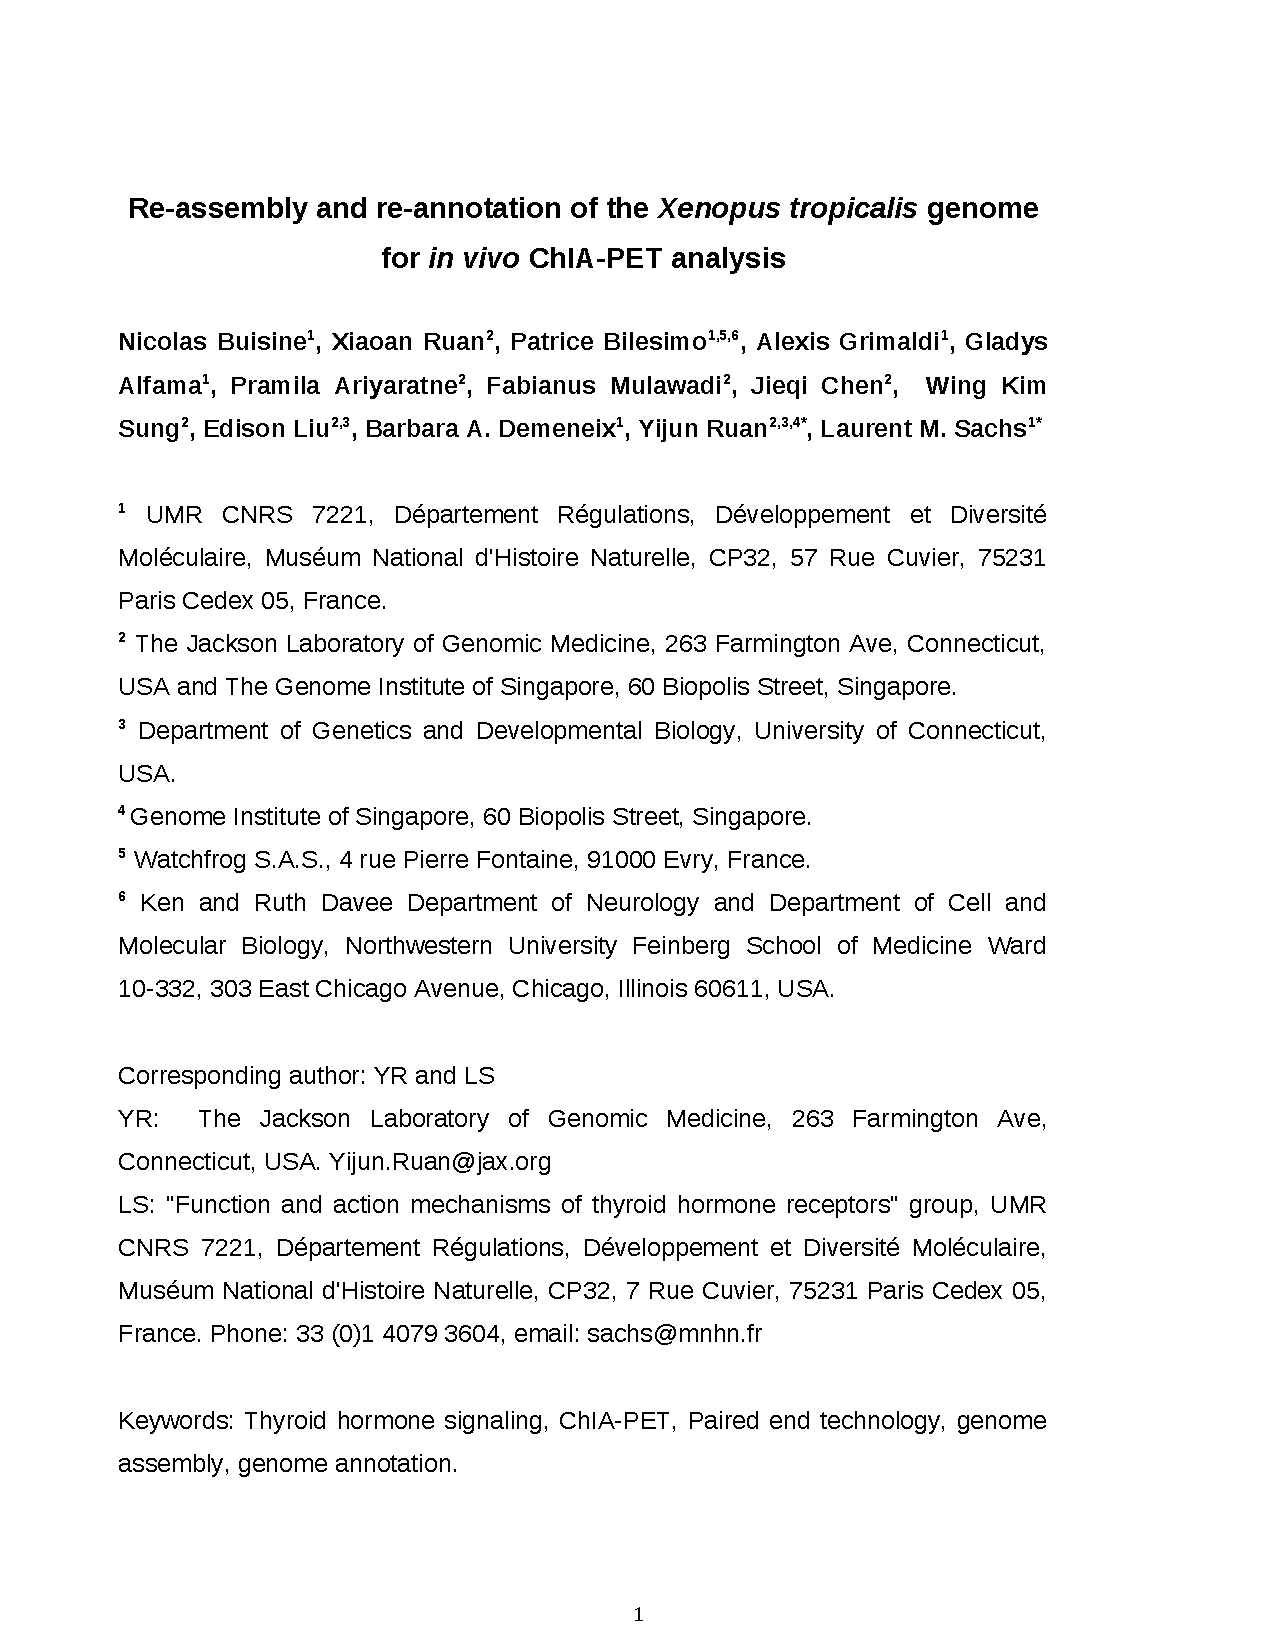
\includepdf[pages={-}]{Publications/buisine2014.pdf}
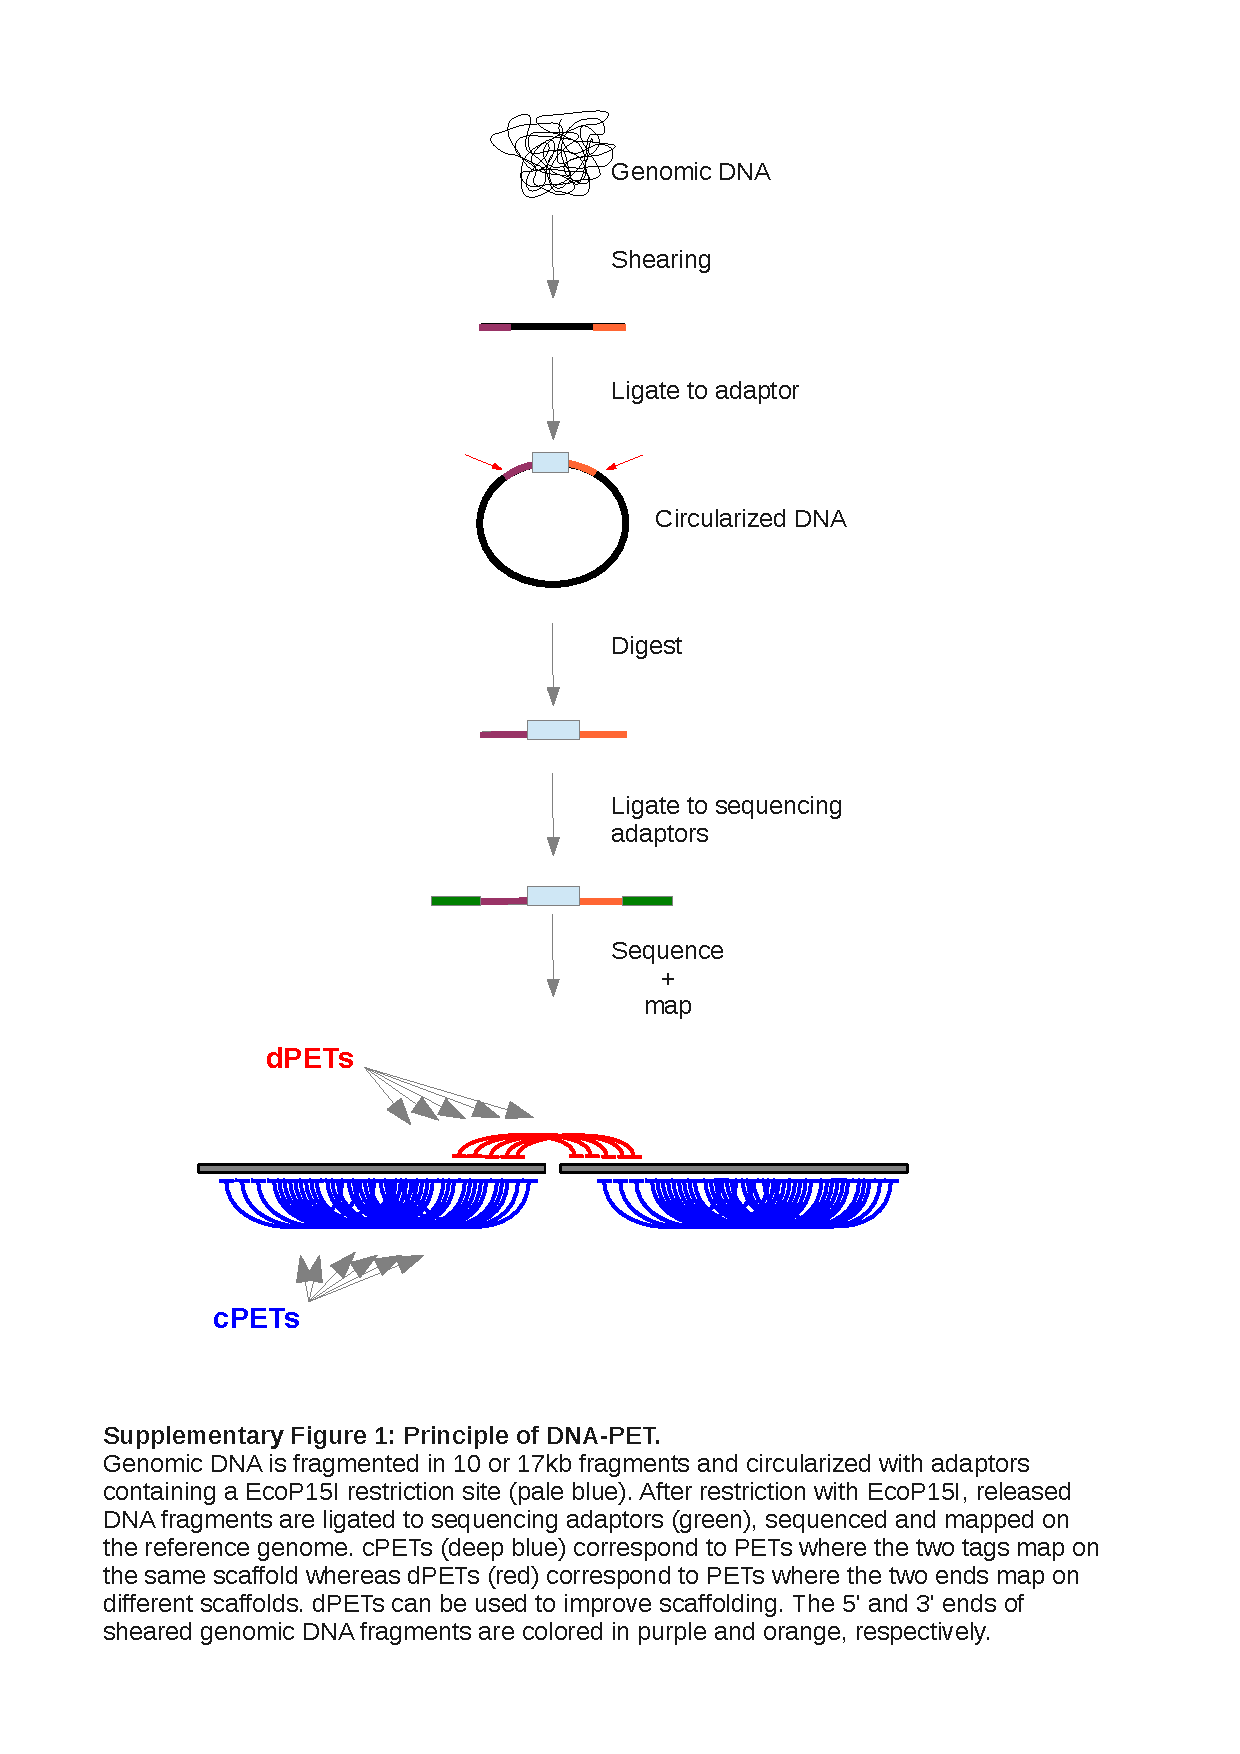
\includepdf[pages={-},nup=1x2,landscape=true]{Publications/buisine2014-sup.pdf}

\end{document}